\subsection{Fully Connected Layers}
\begin{frame}{}
    \LARGE CNN Layer: \textbf{Flattening & Fully Connected Layers}
\end{frame}

\begin{frame}[fragile]{Flattening & Fully Connected Layers}
\begin{block}{Flatten:}
    \begin{itemize}
        \item Flattening is the process of converting a multi-dimensional tensor into a one-dimensional tensor.
        \item Flattening is typically done before passing the data to fully connected layers.
    \end{itemize}
\end{block}

\begin{block}{FC Layer:}
    \begin{itemize}
        \item Used to learn complex relationships between features.
        \item Typically used at the end of the network to make predictions.
        \item Take the flattened output from the previous layer and produce a vector of class scores.
        \item Are often followed by activation functions like ReLU or softmax.
    \end{itemize}
\end{block}

\begin{lstlisting}[language=Python, caption={Code snippet (PyTorch)}, basicstyle=\ttfamily\footnotesize]
import torch.nn as nn
import torch

x = torch.flatten(x, 1)  # preserve batch dim
fc = nn.Linear(in_features=16*8*8, out_features=10)
out = fc(x)
\end{lstlisting}
\end{frame}  

\begin{frame}{CNN - Flattening & Fully Connected Layers}
\begin{figure}
\centering
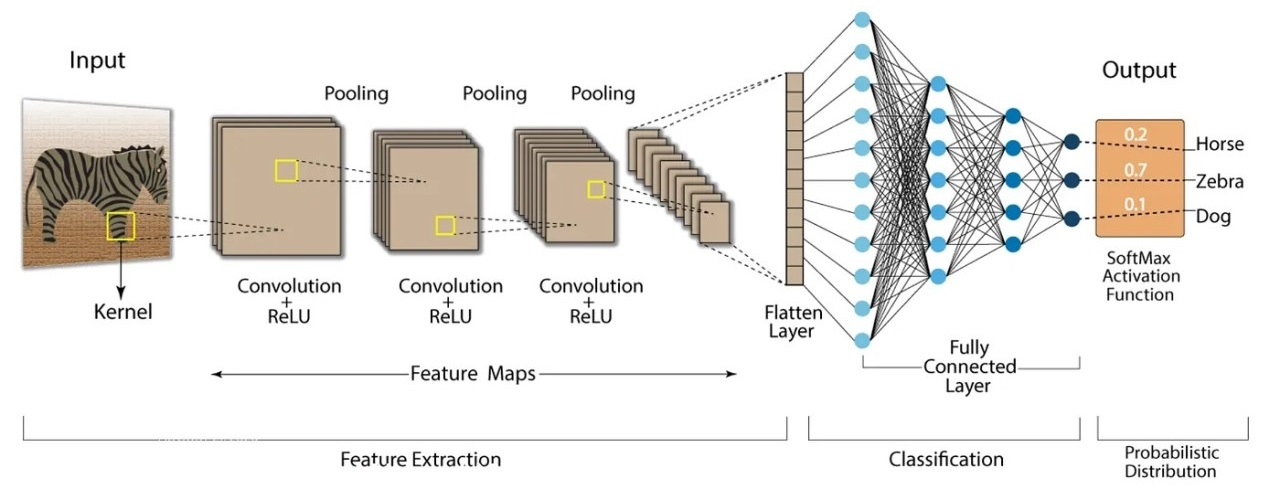
\includegraphics[width=1.0\textwidth,height=0.9\textheight,keepaspectratio]{images/cnn/cnn-fully-connected.jpeg}
\end{figure}
    
\end{frame}